\section{Introduction} \label{sec:Introduction}

It is generally agreed upon that large-scale, universal quantum computing will require comprehensive error correction. One such candidate is the so-called surface code, but the question remains how to physically implement such a system. 

In this report, we will build upon a proposal for a silicon based surface code quantum computer \cite{OGorman2016} and simulate a simple toy model that contains all the essential features. 
The report is structured as follows: In the subsequent sections, we will introduce the surface code and the results obtained by \citet{OGorman2016}. We will then go on review the methods used in the simulation and the choice for materials, which in turn affect the simulation parameters. Following that, we introduce various errors into our model in section \ref{sec:errors} and show how they affect the performance of the system. Finally, we summarise our results in section \ref{sec:conclusion} and provide a number of suggestions as how to this work could be continued. 

\subsection{The surface code}
The surface code is one of the most-well studied fault-tolerant codes \cite{Wang2011,Fowler2012}. Its versatility, large code distance and large fault-tolerance threshold ($1.1\%$) have contributed to various proposals \cite{Fowler2012,Pica2014,Tosi2015,Hill2015,OGorman2016} and some attempts at physical implementation \cite{Barends2014,Kelly2015}. One key aspect of the surface code is its use of vertex and plaquette operators that perform stabiliser measurements on all data qubits using ancillary qubits. If one stabiliser gives a measurement outcome $-1$, it means that these specific four data qubits have undergone an error, whereas a $+1$ outcome indicate that the qubit states are in the codespace. As a consequence, the stabiliser measurements cannot identify errors that correspond to logical operations. At the same time, the stabiliser allow us to actually perform logical operations, which means that a physical implementation of the surface code would not require individual addressing of the data qubits. 

The stabilisers measurements require several data qubits to interact with one ancillary qubit. This probe qubit is then measured, and its outcome is essentially  a measurement parity of four data qubits, that is, whether none or two,  (even parity) one  or three (odd parity) errors have been detected. Of course, the stabiliser measurement can also fail, but this is taken into account in large-scale fault-tolerance calculations. 




\subsection{A physical implementation} \label{sec:PhysicalImplementation}
In 2015, \citet{OGorman2016} proposed a scheme for implementing the surface code in silicon. In this proposal the stabiliser measurements are realised by a mechanical approach, where the data and probe qubit arrays are embedded in two separate layers (see fig.\@ \ref{FIG:paper-mems}). Both layers are brought into close contact ($d\ll D$) and a relative motion of one layer to the other leads to the probe qubits orbiting above the data qubits. This movement allows to perform the stabiliser measurement using a parity measurement where one probe qubit interacts with four data qubits throughout its orbit (see fig.\@ \ref{FIG:paper-parity}). Microelectromechanical systems (MEMS) could be used to implement this motion.


\begin{figure}[H]
	\centering
	\subfloat[]{ 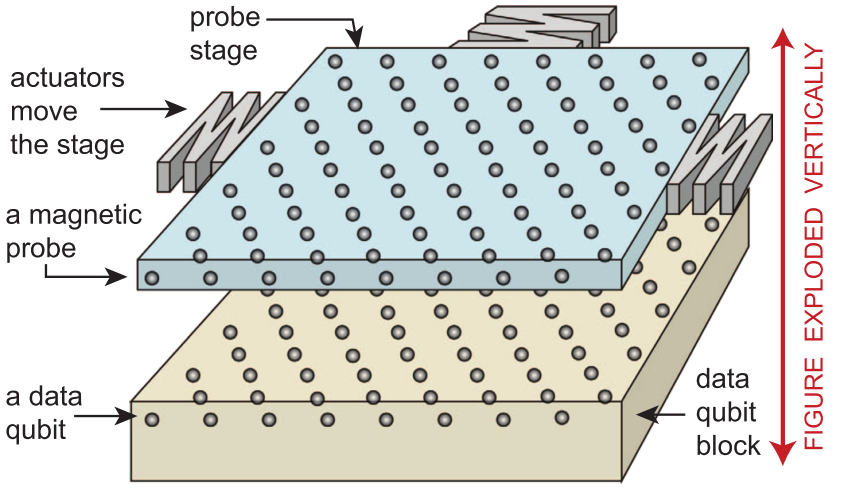
\includegraphics[width=0.8\linewidth]{../Figures/paper-mems} \label{FIG:paper-mems}}\\
	\subfloat[]{ 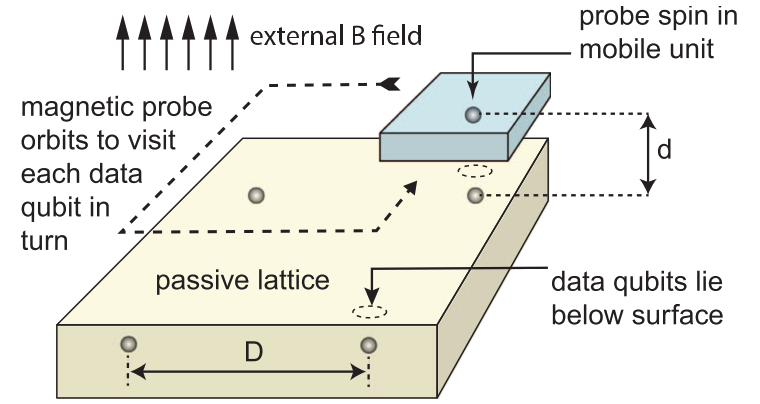
\includegraphics[width=0.8\linewidth]{../Figures/paper-parity} \label{FIG:paper-parity}}
	\caption[paper]{(a) Schematic of a scalable processor where data and ancillary/probe qubits are arranged in arrays in two different layers/stages which are moving relative to each other. (b) Magnified view of four data and one probe qubits. The movement results in the probe qubit orbiting above the data qubits allowing to implement a parity measurement. Direct copy from \cite{OGorman2016}.}
	\label{FIG:paper}
\end{figure}

This scheme requires a high precision in qubit placement. Therefore, \citet{OGorman2016} performed large-scale fault-tolerance simulation to obtain thresholds on the qubit placement precision.

The orbit and movement can be performed in many different ways. \citet{OGorman2016} present results for an abrupt orbit, where the probe qubit is moved rapidly from one data qubit to another, and a smooth, circular orbit.

Several thresholds were obtained with respect where a data qubit displacement distribution is modelled as either a `pillbox' or an ellipsoid shape.
They found reasonable thresholds for each configuration compared to current qubit placement precisions offering good prospects for achieving logical qubit protection at the large scale. 

If we were to implement such a system in the lab, we would probably start with the smallest possible building block, which in this case is the system consisting of four data qubits and a single probe qubit to demonstrate a single parity measurement.
